\documentclass[12pt]{article}
\usepackage{amsmath}
\usepackage{graphicx}
\usepackage{hyperref}
\usepackage{listings}
\usepackage{color}
\usepackage{pythonhighlight}


\title{Operating System Course Report - First Half of the Semester}
\author{B class}
\date{\today}

\begin{document}

\maketitle
\newpage

\tableofcontents
\newpage

\section{Introduction}
This report summarizes the topics covered during the first half of the Operating System course. It includes theoretical concepts, practical implementations, and assignments. The course focuses on the fundamentals of operating systems, including system architecture, process management, CPU scheduling, and deadlock handling.

\section{Course Overview}
\subsection{Objectives}
The main objectives of this course are:
\begin{itemize}
    \item To understand the basic components and architecture of a computer system.
    \item To learn process management, scheduling, and inter-process communication.
    \item To explore file systems, input/output management, and virtualization.
    \item To study the prevention and handling of deadlocks in operating systems.
\end{itemize}

\subsection{Course Structure}
The course is divided into two halves. This report focuses on the first half, which covers:
\begin{itemize}
    \item Basic Concepts and Components of Computer Systems
    \item System Performance and Metrics
    \item System Architecture of Computer Systems
    \item Process Description and Control
    \item Scheduling Algorithms
    \item Process Creation and Termination
    \item Introduction to Threads
    \item File Systems
    \item Input and Output Management
    \item Deadlock Introduction and Prevention
    \item User Interface Management
    \item Virtualization in Operating Systems
\end{itemize}

\section{Topics Covered}

\subsection{Basic Concepts and Components of Computer Systems}
This section explains the fundamental components that make up a computer system, including the CPU, memory, storage, and input/output devices.

\subsection{System Performance and Metrics}
This section introduces various system performance metrics used to measure the efficiency of a computer system, including throughput, response time, and utilization.

\subsection{System Architecture of Computer Systems}
Describes the architecture of modern computer systems, focusing on the interaction between hardware and the operating system.

\subsection{Process Description and Control}
Processes are a central concept in operating systems. This section covers:
\begin{itemize}
    \item Process states and state transitions
    \item Process control block (PCB)
    \item Context switching
\end{itemize}

\subsection{Scheduling Algorithms}
    \subsubsection{First-Come, First-Served (FCFS)} 
    \subsubsection{Shortest Job Next (SJN)}
    \begin{figure}[h]
    \centering
    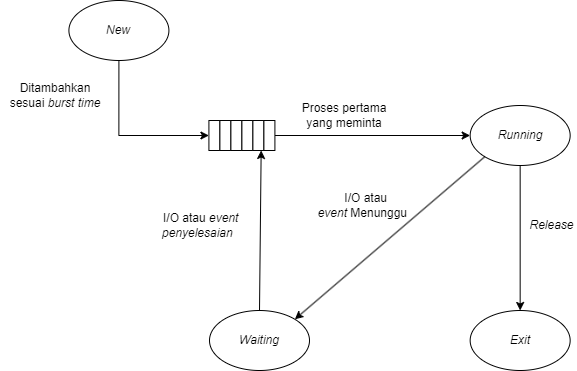
\includegraphics[width=0.75\textwidth]{assets/SJN 2.1.png}
    \label{fig:diagram}
    \end{figure}
     \hspace{1cm} Dalam algoritma \textit{Shortest Job Next} (SJN), saat memilih proses berikutnya yang akan dijalankan, kita melihat semua proses yang berada dalam keadaan siap dan memilih yang memiliki waktu eksekusi paling singkat. Dalam hal ini, kita perlu mengetahui waktu eksekusi setiap proses pada titik waktu tertentu. SJN adalah algoritma \textit{non-preemptive}, artinya proses baru tidak akan mendapatkan giliran di CPU sampai proses yang sedang berjalan selesai, meskipun proses baru memiliki waktu eksekusi yang lebih singkat.

    \hspace{1cm} Dalam algoritma Shortest Job Next (SJN), beberapa istilah kunci perlu dipahami untuk memahami cara kerja algoritma ini. Berikut adalah istilah-istilah yang relevan: 
    
    \begin{itemize}
        \item \textit{Service time} adalah jumlah waktu yang dibutuhkan oleh sebuah proses atau job untuk menyelesaikan eksekusinya setelah mulai berjalan di CPU. \textit{Service time} juga dikenal sebagai burst time.
        \item \textit{Arrival time} adalah waktu ketika sebuah proses tiba dan siap untuk dieksekusi di CPU atau antrian penjadwalan.
        \item \textit{Completion time} adalah titik waktu ketika sebuah proses menyelesaikan eksekusinya.
        \item \textit{Turnaround time} adalah total waktu yang dibutuhkan oleh sebuah proses untuk menyelesaikan eksekusinya, dari saat proses tersebut tiba di antrian \textit{ready} hingga selesai dieksekusi. \textit{Turnaround time} dihitung sebagai \textit{completion time} dikurangi \textit{arrival time}.
        \item Algoritma penjadwalan \textit{non-preemptive} adalah  algoritma yang sebuah proses yang telah mulai dieksekusi akan terus berjalan sampai selesai. Proses baru tidak diizinkan untuk mengganggu proses yang sedang berjalan. 
    \end{itemize}
    
     \hspace{1cm}Penggunaan algoritma SJN memiliki beberapa keuntungan yang signifikan. Berikut adalah beberapa keuntungan utama dari SJN:
     \begin{enumerate}
         \item Penjadwalan SJN meminimalkan waktu tunggu rata-rata untuk proses di antrian \textit{ready} karena proses yang lebih singkat diberi prioritas lebih tinggi, sehingga mengurangi waktu tunggu mereka dan meningkatkan kinerja sistem dalam hal waktu respons dan penyelesaian (\textit{turnaround time}).
         \item Penggunaan algoritma \textit{Shortest Job Next} (SJN) dapat meningkatkan pemanfaatan sumber daya CPU karena algoritma ini memprioritaskan proses yang lebih pendek. Hal ini memungkinkan lebih banyak proses untuk diselesaikan dengan lebih cepat.
     \end{enumerate}
     
    \hspace{1cm}Meskipun SJN memiliki keuntungan, terdapat juga beberapa kerugian yang perlu diperhatikan. Berikut adalah beberapa kerugian utama dari algoritma SJN:
    \begin{itemize}
        \item \textit{Starvation} dapat menjadi masalah dalam penggunaan algoritma SJN. Dalam situasi ini, proses dengan durasi lebih lama mungkin tidak pernah mendapatkan kesempatan untuk dieksekusi jika ada kedatangan proses yang lebih pendek secara terus-menerus. Ini bisa menjadi masalah terutama dalam sistem yang mengutamakan keadilan.
        \item Memperkirakan durasi proses dengan akurat bisa menjadi tugas yang sulit dalam praktiknya. Jika perkiraan durasi proses ternyata tidak akurat, hal ini bisa memengaruhi kinerja SJN dan menyebabkan preemption yang sering.
        \item Dalam situasi ketika respons cepat sangat penting, SJN mungkin bukan pilihan yang paling responsif untuk sistem interaktif atau lingkungan \textit{real-time}. Ketika proses singkat mendominasi CPU, proses yang lebih panjang bisa mengalami penundaan yang lama, yang sering kali merugikan.
    \end{itemize}

    Algoritma SJN memiliki karakteristik unik yang membedakannya dari algoritma penjadwalan lainnya. Berikut adalah beberapa karakteristik dari SJN:
    \begin{itemize}
        \item \textit{Shortest Job Next} memiliki keuntungan berupa waktu tunggu rata-rata yang minimum dibandingkan dengan semua algoritma penjadwalan lainnya.
        \item Algoritma ini merupakan \textit{Greedy Algorithm}, yang berarti mengambil keputusan yang terbaik saat ini tanpa mempertimbangkan konsekuensi di masa depan.
        \item Algoritma ini dapat menyebabkan \textit{starvation} jika proses yang lebih pendek terus menerus muncul. Masalah ini dapat diatasi dengan menggunakan konsep \textit{ageing}, yaitu memberikan prioritas kepada proses yang telah menunggu lebih lama.
        \item Dalam praktiknya, SJN sulit diterapkan karena sistem operasi mungkin tidak mengetahui \textit{burst time} dan karena itu tidak dapat mengurutkannya. Meskipun tidak mungkin untuk memprediksi waktu eksekusi dengan akurat, beberapa metode dapat digunakan untuk memperkirakan waktu eksekusi suatu \textit{job}, seperti menggunakan rata-rata tertimbang dari waktu eksekusi sebelumnya.
        \item SJN dapat digunakan di lingkungan khusus jika perkiraan waktu \textit{running} akurat tersedia.
    \end{itemize}
    \begin{figure}[h]
    \centering
    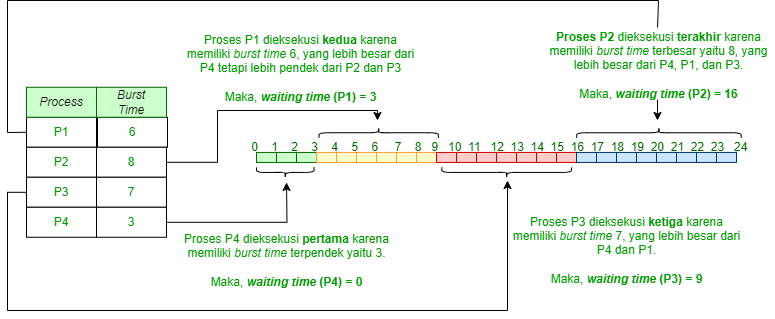
\includegraphics[width=0.75\textwidth]{assets/SJN 2.2.png}
    \label{fig:diagram}
    \end{figure}
    Berikut adalah langkah-langkah dalam algoritma \textit{Shortest Job Next} (SJN):
    \begin{enumerate} 
        \item Urutkan semua proses berdasarkan \textit{arrival time}.
        \item Pilih proses yang memiliki \textit{arrival time} terkecil dan \textit{burst time} terkecil.
        \item Setelah proses tersebut selesai, buat kumpulan proses (\textit{pool}) yang tiba setelahnya hingga proses sebelumnya selesai.
        \item Dari kumpulan tersebut, pilih proses yang memiliki \textit{burst time} terkecil untuk dieksekusi selanjutnya.
    \end{enumerate}
    Referensi:\\
    GeeksforGeeks. (n.d.-c). Shortest Job Next (SJN) in Operating System. Retrieved October 1, 2024, from https://www.geeksforgeeks.org/shortest-job-next-sjn-in-operating-system/

    GeeksforGeeks. (n.d.-d). Program for Shortest Job First (SJF) CPU scheduling | Set 1 (non-preemptive). Retrieved October 1, 2024, from https://www.geeksforgeeks.org/program-for-shortest-job-first-or-sjf-cpu-scheduling-set-1-non-preemptive/

    \subsubsection{Round Robin (RR)} 


\subsection{Process Creation and Termination}
Details how processes are created and terminated by the operating system, including:
\begin{itemize}
    \item Process spawning
    \item Process termination conditions
\end{itemize}

\subsection{Introduction to Threads}
This section introduces the concept of threads and their relation to processes, covering:
\begin{itemize}
    \item Single-threaded vs. multi-threaded processes
    \item Benefits of multithreading
\end{itemize}

\subsection{File Systems}
File systems provide a way for the operating system to store, retrieve, and manage data. This section explains:
\begin{itemize}
    \item File system structure
    \item File access methods
    \item Directory management
\end{itemize}

\subsection{Input and Output Management}
Input and output management is key for handling the interaction between the system and external devices. This section includes:
\begin{itemize}
    \item Device drivers
    \item I/O scheduling
\end{itemize}

\subsection{Deadlock Introduction and Prevention}
Explores the concept of deadlocks and methods for preventing them:
\begin{itemize}
    \item Deadlock conditions
    \item Deadlock prevention techniques
\end{itemize}

\subsection{User Interface Management}
This section discusses the role of the operating system in managing the user interface. Topics covered include:
\begin{itemize}
    \item Graphical User Interface (GUI)
    \item Command-Line Interface (CLI)
    \item Interaction between the user and the operating system
\end{itemize}

\subsection{Virtualization in Operating Systems}
Virtualization allows multiple operating systems to run concurrently on a single physical machine. This section explores:
\begin{itemize}
    \item Concept of virtualization
    \item Hypervisors and their types
    \item Benefits of virtualization in modern computing
\end{itemize}

\section{Assignments and Practical Work}
\subsection{Assignment 1: Process Scheduling}
Students were tasked with implementing various process scheduling algorithms (e.g., FCFS, SJN, and RR) and comparing their performance under different conditions.

\subsection{Assignment 2: Deadlock Handling}
In this assignment, students were asked to simulate different deadlock scenarios and explore various prevention methods.

\subsection{Assignment 3: Multithreading and Amdahl's Law}
This assignment involved designing a multithreading scenario to solve a computationally intensive problem. Students then applied **Amdahl's Law** to calculate the theoretical speedup of the program as the number of threads increased.

\subsection{Assignment 4: Simple Command-Line Interface (CLI) for User Interface Management}
Students were tasked with creating a simple **CLI** for user interface management. The CLI should support basic commands such as file manipulation (creating, listing, and deleting files), process management, and system status reporting.
\subsubsection{Group 5}
soal:\\
Buatlah program Command-Line Interface (CLI) sederhana dalam Python dengan fitur-fitur berikut:
\begin{itemize}
    \item list files: Menampilkan semua file yang ada di direktori saat ini.
    \item create file: membuat file baru dengan nama yang ditentukan
    \item delete file: Menghapus file berdasarkan nama yang diberikan, jika file tersebut ada.
    \item process list: Menampilkan daftar proses yang sedang berjalan beserta PID dan nama proses.
    \item system status: Menampilkan status sistem saat ini, termasuk penggunaan CPU dan memori.
    \item exit: Menghentikan program CLI.
\end{itemize}
\begin{python}
import os
import psutil

def create_file(filename):
    with open(filename, 'w') as file:
        file.write(input("Masukkan teks untuk file baru: "))
    print(f"File '{filename}' berhasil dibuat.")

def list_files():
    files = os.listdir()
    print("Daftar file dalam direktori saat ini:")
    for file in files:
        print(file)

def delete_file(filename):
    try:
        os.remove(filename)
        print(f"File '{filename}' berhasil dihapus.")
    except FileNotFoundError:
        print(f"File '{filename}' tidak ditemukan.")

def list_processes():
    for proc in psutil.process_iter(['pid', 'name']):
        print(f"PID: {proc.info['pid']}, Nama: {proc.info['name']}")

def kill_process(pid):
    try:
        p = psutil.Process(pid)
        p.terminate()
        print(f"Proses dengan PID {pid} berhasil dihentikan.")
    except psutil.NoSuchProcess:
        print(f"Tidak ada proses dengan PID {pid}.")

def system_status():
    cpu_usage = psutil.cpu_percent(interval=1)
    memory_info = psutil.virtual_memory()
    print(f"Penggunaan CPU: {cpu_usage}%")
    print(f"Penggunaan Memori: {memory_info.percent}%")

# Main CLI
while True:
    print("Masukkan Perintah:\n1. create_files\n2. list_files\n3. delete_file\n4. list_process\n5. kill_process\n6. system_status\n6. exit\n")
    command = input("Masukkan perintah: ").split()
    if command[0] == "create_file":
        create_file(command[1])
    elif command[0] == "list_files":
        list_files()
    elif command[0] == "delete_file":
        delete_file(command[1])
    elif command[0] == "list_processes":
        list_processes()
    elif command[0] == "kill_process":
        kill_process(int(command[1]))
    elif command[0] == "system_status":
        system_status()
    elif command[0] == "exit":
        print("Keluar dari CLI")
        break
    else:
        print("Perintah tidak dikenal.")
\end{python}

\subsection{Assignment 5: File System Access}
In this assignment, students implemented file system access routines, including:
\begin{itemize}
    \item File creation and deletion
    \item Reading from and writing to files
    \item Navigating directories and managing file permissions
\end{itemize}
\subsubsection{Group 5}
Soal:\\
Buatlah sebuah program manajemen file sederhana dengan Python yang memiliki fitur sebagai berikut:
\begin{itemize}
    \item Create file: Meminta pengguna memasukkan nama file dan kontennya untuk dibuat.
    \item Read file: Membaca dan menampilkan isi dari file berdasarkan nama yang diberikan pengguna.
    \item Delete file: Menghapus file yang namanya diberikan oleh pengguna.
    \item List files: Menampilkan semua file dalam direktori saat ini tanpa meminta input tambahan.
    \item Exit: Menghentikan program.
\end{itemize}
Program harus terus berjalan hingga pengguna memilih opsi Exit. Buat menu interaktif dengan pilihan 1-5 untuk setiap operasi di atas, dan tampilkan pesan yang sesuai jika file tidak ditemukan atau format input salah.
\begin{python}
    import os

# 1. Fungsi untuk membuat file dan menulis konten ke dalamnya
def create_file(filename, content):
    with open(filename, 'w') as file:
        file.write(content)
    print(f"File '{filename}' berhasil dibuat.")

# 2. Fungsi untuk membaca konten file
def read_file(filename):
    if os.path.exists(filename):
        with open(filename, 'r') as file:
            content = file.read()
            print(f"Isi file '{filename}':\n{content}")
    else:
        print(f"File '{filename}' tidak ditemukan.")

# 3. Fungsi untuk menghapus file
def delete_file(filename):
    if os.path.exists(filename):
        os.remove(filename)
        print(f"File '{filename}' berhasil dihapus.")
    else:
        print(f"File '{filename}' tidak ditemukan.")

# 4. Fungsi untuk menampilkan daftar file di direktori tertentu
def list_files(directory):
    if os.path.isdir(directory):
        files = os.listdir(directory)
        print(f"Daftar file di '{directory}':")
        for file in files:
            print(f"- {file}")
    else:
        print(f"Direktori '{directory}' tidak ditemukan.")

# Menu utama untuk menerima input dari pengguna
while True:
    print("\nPilih operasi yang ingin dilakukan:")
    print("1. Create file")
    print("2. Read file")
    print("3. Delete file")
    print("4. List files")
    print("5. Exit")
    choice = input("Masukkan pilihan (1-5): ")

    if choice == "1":
    #     # Operasi create file
        file_data = input("Masukkan nama file dan isi konten (format: 'nama_file,konten_file'): ")
         # Memisahkan nama file dan konten
        if ',' in file_data:
            filename, content = file_data.split(',', 1)  # Split at the first comma only
            filename = filename.strip()
            content = content.strip()
            create_file(filename, content)
        else:
            print("Input tidak valid. Pastikan menggunakan format: 'nama_file,konten_file' tanpa spasi atau dengan spasi.")
        
    elif choice == "2":
        # Operasi read file
        filename = input("Masukkan nama file yang ingin dibaca: ")
        read_file(filename.strip())
        
    elif choice == "3":
        # Operasi delete file
        filename = input("Masukkan nama file yang ingin dihapus: ")
        delete_file(filename.strip())
        
    elif choice == "4":
        # Operasi list files
        list_files(".")
        
    elif choice == "5":
        # Keluar dari program
        print("Terima kasih! Program dihentikan.")
        break
        
    else:
        print("Pilihan tidak valid, silakan coba lagi.")
\end{python}

\section{Conclusion}
The first half of the course introduced core operating system concepts, including process management, scheduling, multithreading, and file system access. These topics provided a foundation for more advanced topics to be covered in the second half of the course.

\end{document}